\documentclass[tikz]{standalone}

\usepackage{mathrsfs}
\begin{document}
	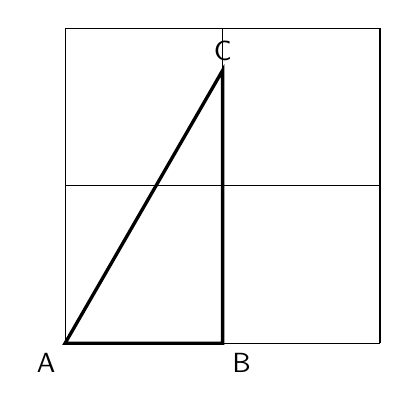
\begin{tikzpicture}[scale=2]
	\draw (0,0) grid (2,2);
	\coordinate[label=below left:$\mathsf{A}$] (A) at (0, 0);
	\coordinate[label=below right:$\mathsf{B}$] (B) at (1, 0);
	\coordinate[label=above:$\mathsf{C}$] (C) at (1, {sqrt(3)});
	\draw[very thick] (C) -- (A) -- (B) -- (C) -- cycle; 
	\end{tikzpicture}
\end{document}